% Created 2021-06-27 Sun 16:31
% Intended LaTeX compiler: pdflatex
\documentclass[11pt]{article}
\usepackage[utf8]{inputenc}
\usepackage[T1]{fontenc}
\usepackage{graphicx}
\usepackage{grffile}
\usepackage{longtable}
\usepackage{wrapfig}
\usepackage{rotating}
\usepackage[normalem]{ulem}
\usepackage{amsmath}
\usepackage{textcomp}
\usepackage{amssymb}
\usepackage{capt-of}
\usepackage{hyperref}
\graphicspath{{../../books/}}
% TIPS
% \substack{a\\b} for multiple lines text





% pdfplots will load xolor automatically without option
\usepackage[dvipsnames]{xcolor}

\usepackage{forest}
% two-line text in node by [two \\ lines]
% \begin{forest} qtree, [..] \end{forest}
\forestset{
  qtree/.style={
    baseline,
    for tree={
      parent anchor=south,
      child anchor=north,
      align=center,
      inner sep=1pt,
    }}}
%\usepackage{flexisym}
% load order of mathtools and mathabx, otherwise conflict overbrace

\usepackage{mathtools}
%\usepackage{fourier}
\usepackage{pgfplots}
\usepackage{amsthm, mathabx,  amsmath, commath}
\usepackage{amsfonts}

\usepackage{empheq}
\usepackage{tikz}
\usetikzlibrary{arrows.meta}
\usepackage[most]{tcolorbox}

\newtheorem{theorem}{Theorem}[section]
\newtheorem{definition}{Definition}[section]
\newtheorem{corollary}{Corollary}[section]
\newtheorem{example}{Example}[section]
\newtheorem{lemma}{Lemma}[section]
\newtheorem{proposition}{Proposition}[section]

\newcommand{\bl}[1] {\boldsymbol{#1}}
\newcommand{\Wt}[1] {\stackrel{\sim}{\smash{#1}\rule{0pt}{1.1ex}}}
\newcommand{\wt}[1] {\widetilde{#1}}


%For boxed texts in align, use Aboxed{}
%otherwise use boxed{}

\DeclareMathSymbol{\widehatsym}{\mathord}{largesymbols}{"62}
\newcommand\lowerwidehatsym{%
  \text{\smash{\raisebox{-1.3ex}{%
    $\widehatsym$}}}}
\newcommand\fixwidehat[1]{%
  \mathchoice
    {\accentset{\displaystyle\lowerwidehatsym}{#1}}
    {\accentset{\textstyle\lowerwidehatsym}{#1}}
    {\accentset{\scriptstyle\lowerwidehatsym}{#1}}
    {\accentset{\scriptscriptstyle\lowerwidehatsym}{#1}}
}

\usepackage{graphicx}
    
% text on arrow for xRightarrow
\makeatletter
%\newcommand{\xRightarrow}[2][]{\ext@arrow 0359\Rightarrowfill@{#1}{#2}}
\makeatother


\def \bx {\boldsymbol{x}}
\def \ba {\boldsymbol{a}}
\def \bI {\boldsymbol{I}}
\def \bt {\boldsymbol{t}}
\def \bb {\boldsymbol{b}}
\def \bA {\boldsymbol{A}}
\def \bX {\boldsymbol{X}}
\def \bu {\boldsymbol{u}}
\def \bS {\boldsymbol{S}}
\def \bZ {\boldsymbol{Z}}
\def \bz {\boldsymbol{z}}
\def \by {\boldsymbol{y}}
\def \bw {\boldsymbol{w}}
\def \bT {\boldsymbol{T}}
\def \bS {\boldsymbol{S}}
\def \bm {\boldsymbol{m}}
\def \bW {\boldsymbol{W}}
\def \bY {\boldsymbol{Y}}
\def \bH {\boldsymbol{H}}
\def \blambda {\boldsymbol{\lambda}}
\def \bPhi {\boldsymbol{\Phi}}
\def \btheta {\boldsymbol{\theta}}
\def \bmu {\boldsymbol{\mu}}
\def \bphi {\boldsymbol{\phi}}
\def \bSigma {\boldsymbol{\Sigma}}
\def \lb {\left\{}
\def \rb {\right\}}
\def \caln {\mathcal{N}}
\def \dissum {\displaystyle\Sigma}
\def \dispro {\displaystyle\prod}
\def \E {\mathbb{E}}
\def \Q {\mathbb{Q}}
\def \V {\mathbb{V}}
\def \R {\mathbb{R}}
\def \calq {\mathcal{Q}}
\def \calg {\mathcal{G}}
\def \caln {\mathcal{N}}
\def \calr {\mathcal{R}}
\def \calm {\mathcal{M}}
\def \calc {\mathcal{C}}
\def \bcup {\bigcup}

\author{Munkres}
\date{\today}
\title{Topology}
\hypersetup{
 pdfauthor={Munkres},
 pdftitle={Topology},
 pdfkeywords={},
 pdfsubject={},
 pdfcreator={Emacs 27.2 (Org mode 9.5)}, 
 pdflang={English}}
\begin{document}

\maketitle
\tableofcontents


\section{Topological Spaces and Continuous Functions}
\label{sec:orgbe1fae9}

\subsection{Topological Spaces}
\label{sec:orga5827aa}
\begin{definition}[]
A \textbf{topology} on a set is a collection \(\calt\) of subsets of \(X\) having the following properties
\begin{enumerate}
\item \(\emptyset\) and \(X\) are in \(\calt\)
\item The union of the elements of any subcollection of \(\calt\) is in \(T\)
\item The intersection of the elements of any finite subcollection of \(\calt\) is in \(\calt\)
\end{enumerate}


A set \(X\) for which a topology \(\calt\) has been specified is called a \textbf{topological space}
\end{definition}

\begin{examplle}[]
Consider \(\bigcap_{n\in\N}(-\frac{1}{n},\frac{1}{n})=\{0\}\). \((-1/n,1/n)\) is open but \(\{0\}\) is not
open in \(\R\).
\end{examplle}

If \(X\)is a topological space with topology \(\calt\), we say that a subset \(U\) of \(X\) is an
\textbf{open set} of \(X\) if \(U\in\calt\)

\begin{examplle}[]
If \(X\) is any set, the collection of all subsets of \(X\) is a topology on \(X\); it is called
the \textbf{discrete topology}. The collection consisting of \(X\) and \(\emptyset\) only is also a topology
on \(X\); we shall call it the \textbf{indiscrete topology}
\end{examplle}

\begin{examplle}[]
Let \(X\) be a set; let \(\calt_f\) be the collection of all subsets \(U\) of \(X\)s.t. \(X-U\)
either is finite or is all of \(X\). Then \(\calt_f\) is a topology on \(X\), called the \textbf{finite
complement topology}. If \(\{U_\alpha\}\) is an indexed family of nonempty elements of \(\calt_f\).
\begin{equation*}
X-\bigcup U_\alpha=\bigcap(X-U_\alpha)
\end{equation*}
\end{examplle}


\begin{definition}[]
Suppose that \(\calt\) and \(\calt'\) are two topology on a given set \(X\). If \(\calt'\supset\calt\) we say
that \(\calt'\) is \textbf{finer} than \(\calt\); if \(\calt'\) properly contains \(\calt\) we say that \(\calt'\)  is
\textbf{strictly finer} than \(\calt\). We say that \(\calt\) is \textbf{coarser} than \(\calt'\) or \textbf{strictly coarser}. We
say \(\calt\) is \textbf{comparable} with \(\calt\) is either \(\calt'\supset\calt\) or \(\calt\supset\calt'\)
\end{definition}

\subsection{Basis for a Topology}
\label{sec:org447db0b}
\begin{definition}[]
If \(X\) is a set, a \textbf{basis} for a topology on \(X\) is a collection \(\calb\) of subsets of \(X\)
(called \textbf{basis element}) s.t.
\begin{enumerate}
\item for each \(x\in X\), there is at least one basis element \(B\) s.t. \(x\in B\)
\item if \(x\in B_1\cap B_2\), then there is a basis element \(B_3\) s.t. \(x\in B_3\subset B_1\cap B_2\)
\end{enumerate}


If \(\calb\) satisfies these conditions, then we define the \textbf{topology \(\calt\) generated by \(\calb\)} as
follows: A subset \(U\) of \(X\) is said to be open in \(X\) if for each \(x\in U\), there is a
basis \(B\in\calb\) s.t. \(x\in B\subset U\).
\end{definition}

Now we show that \(\calt\) is indeed a topology. Take an indexed family \(\{U_\alpha\}_{\alpha\in J}\) of elements
of \(\calt\), we show that
\begin{equation*}
U=\bigcup_{\alpha\in J}U_\alpha
\end{equation*}
belongs to \(\calt\). Given \(x\in U\), there is an index \(\alpha\) s.t. \(x\in U_\alpha\). Since \(U_\alpha\) is open,
there is a basis element \(B\) s.t. \(x\in B\subset U_\alpha\). Then \(x\in B\) and \(B\subset U\), so \(U\) is open.

If \(U_1,U_2\in \calt\), then given \(x\in U_1\cap U_2\). we choose \(x\in B_1\subset U_1\) and \(x\in B_2\subset U_2\). By the
second condition  for a basis we have \(x\in B_3\subset B_1\cap B_2\). Hence \(x\in B_3\subset U_1\cap U_2\).

\begin{lemma}[]
Let \(X\) be a set; let \(\calb\) be a basis for a topology \(\calt\) on \(X\). Then \(\calt\) equals the
collection of all unions of elements of \(\calb\).
\end{lemma}

\begin{proof}
Given a collection of elements of \(\calb\), they are also elements of \(\calt\). Because \(\calt\) is a
topology, their union is in \(\calt\).

Conversely, given \(U\in\calt\), choose for each \(x\in U\) an element \(B_x\) for \(B\)
s.t. \(x\in B_x\subset U\). Then \(U=\bigcup_{x\in U}B_x\)
\end{proof}

\begin{lemma}[]
\label{lemma13.2}
Let \(X\) be a topological space. Suppose that \(\calc\) is a collection of open sets of \(X\) s.t.
for each open set \(U\) of \(X\) and each \(x\) in \(U\), there is an element \(C\) of \(\calc\)
s.t. \(x\in C\subseteq U\). Then \(\calc\) is a basis for the topology of \(X\).
\end{lemma}

\begin{proof}
Let \(x\in C_1\cap C_2\), since \(C_1\) and \(C_2\) is open, \(C_1\cap C_2\) is open. Hence there
exists \(C_3\in\calc\) s.t. \(x\in C_3\subseteq C_1\cap C_2\)

Let \(\calt\) be the collection of open sets of \(X\); we must show that the topology \(\calt'\)
generated by \(\calc\) equals the topology \(\calt\). If \(U\in\calt\), then there is \(x\in C\subset U\). If \(W\in\calt'\),
then \(W=\bigcup_{x\in W} B_x\) and \(B_x\in\calt\)
\end{proof}

\begin{lemma}[]
Let \(\calb\) and \(\calb'\) be bases for the topologies \(\calt\) and \(\calt'\), respectively, on \(X\). TFAW
\begin{enumerate}
\item \(\calt'\) is finer than \(\calt\)
\item For each \(x\in X\) and each basis element \(x\in B\in\calb\) there is a basis element \(B'\in\calb'\)
s.t. \(x\in B'\subset B\)
\end{enumerate}
\end{lemma}

\begin{proof}
\(2\to1\). Given \(U\in\calt\). Then \(x\in B\subset U\) and \(x\in B'\subset U\). Hence \(U\in\calt'\).

\(1\to 2\). given \(x\in B\in\calb\). Since \(\calt\subset\calt'\) we have \(B\in\calt'\). Since \(\calt'\) is generated by \(\calb'\)
there is an element \(B'\in\calb'\) s.t. \(x\in B'\subset B\)
\end{proof}

\begin{definition}[]
If \(\calb\) is the collection of all open intervals in the real line
\begin{equation*}
(a,b)=\{x\mid a<x<b\}
\end{equation*}
the topology generated by \(\calb\) is called the \textbf{standard topology} on the real line. If \(\calb'\) is
the collection of all half-opne intervals of the form
\begin{equation*}
[a,b)=\{x\mid a\le x<b\}
\end{equation*}
where \(a<b\), the topology generated by \(\calb'\) is called the \textbf{lower limit topology} of \(\R\).
When \(\R\) is given the lower limit topology, we denote it by \(\R_l\). Finally let \(K\) denote
the set of all numbers of the form \(1/n\) for \(n\in\Z_+\), and let \(\calb''\) be the collection of all
open intervals \((a,b)\) along with all sets of the form \((a,b)-K\). The topology generated
by \(\calb''\) is called the \textbf{\(K\)-topology} on \(R\). When \(\R\) is given this topology, we denote it
by \(\R_K\)
\end{definition}

\begin{lemma}[]
The topologies of \(\R_l\) and \(\R_K\) are strictly finer than the standard topology on \(\R\), but
are not comparable with one another.
\end{lemma}

\begin{proof}
Let \(\calt,\calt',\calt''\) be the topologies of \(\R,\R_l,\R_K\). Given a basis element \((a,b)\) for \(\calt\)
and a point \(x\) of \((a,b)\), the basis element \(x\in[x,b)\subset(a,b)\). On the other hand, given the
basis element \([x,d)\in\calt\)  there is no interval \((a,b)\) that contains \(x\) and lies
in \([x,d)\). Thus \(\calt\) is strictly finer than \(\calt\).

Given \(B=(-1,1)-K\in\calt''\) and the point 0 of \(B\), there is no open interval of \(\calt\) that
contains 0 and lies in \(B\)

Also given \(B\), there is no \([x,b)\in\calt'\)  s.t. \([x,b)\subset B\).
\end{proof}

\begin{definition}[]
A \textbf{subbasis} \(\cals\) for a topology on \(X\) is a collection of subsets of \(X\) whose union
equals \(X\). The \textbf{topology generated by the subbasis} \(\cals\) is defined to be the collection \(\calt\)
of all unions of finite intersection of elements of \(\cals\).
\end{definition}

\subsection{The Order Topology}
\label{sec:org135dfd1}
Given elements \uline{\(a\) and \(b\) of \(X\)} s.t. \(a<b\),\((a,b)\),\((a,b]\),\([a,b)\) and \([a,b]\)
are \textbf{intervals}

\begin{definition}[]
Let \(X\) be a set with a simple order relation; assume \(X\) has more than one element.
Let \(\calb\) be the collection of all sets of the following types:
\begin{enumerate}
\item All open intervals \((a,b)\) in \(X\)
\item All intervals of the form \([a_0,b)\) where \(a_0\) is the smallest element of \(X\)
\item All intervals of the form \((a,b_0]\) where \(b_0\) is the largest element of \(X\)
\end{enumerate}


The collection \(\calb\) is a basis for a topology on \(X\), which is called the \textbf{order topology}
\end{definition}


\subsection{The Product Topology on \texorpdfstring{$X\times Y$}{X Y}}
\label{sec:org41146b6}

\begin{definition}[]
Let \(X\) and \(Y\) be topological spaces. The \textbf{product topology} on \(X\times Y\) is the topology
having as basis the collection \(\calb\) of all sets of the form \(U\times V\), where \(U\) is an open
subset of \(X\) and \(V\) is an open subset of \(Y\)
\end{definition}

\begin{theorem}[]
If \(\calb\) is a basis for the topology of \(X\) and \(\calc\) is a basis for the topology of \(Y\),
then the collection
\begin{equation*}
\cald=\{B\times C\mid B\in\calb\text{ and }C\in\calc\}
\end{equation*}
is a basis for the topology of \(X\times Y\)
\end{theorem}


\begin{theorem}[]
The collection
\begin{equation*}
\cals=\{\pi_1^{-1}(U)\mid U\text{ open in }X\}\cup\{\pi_2^{-1}(V)\mid V\text{ open in }Y\}
\end{equation*}
is a subbasis for the product topology on \(X\times Y\)
\end{theorem}

\begin{center}
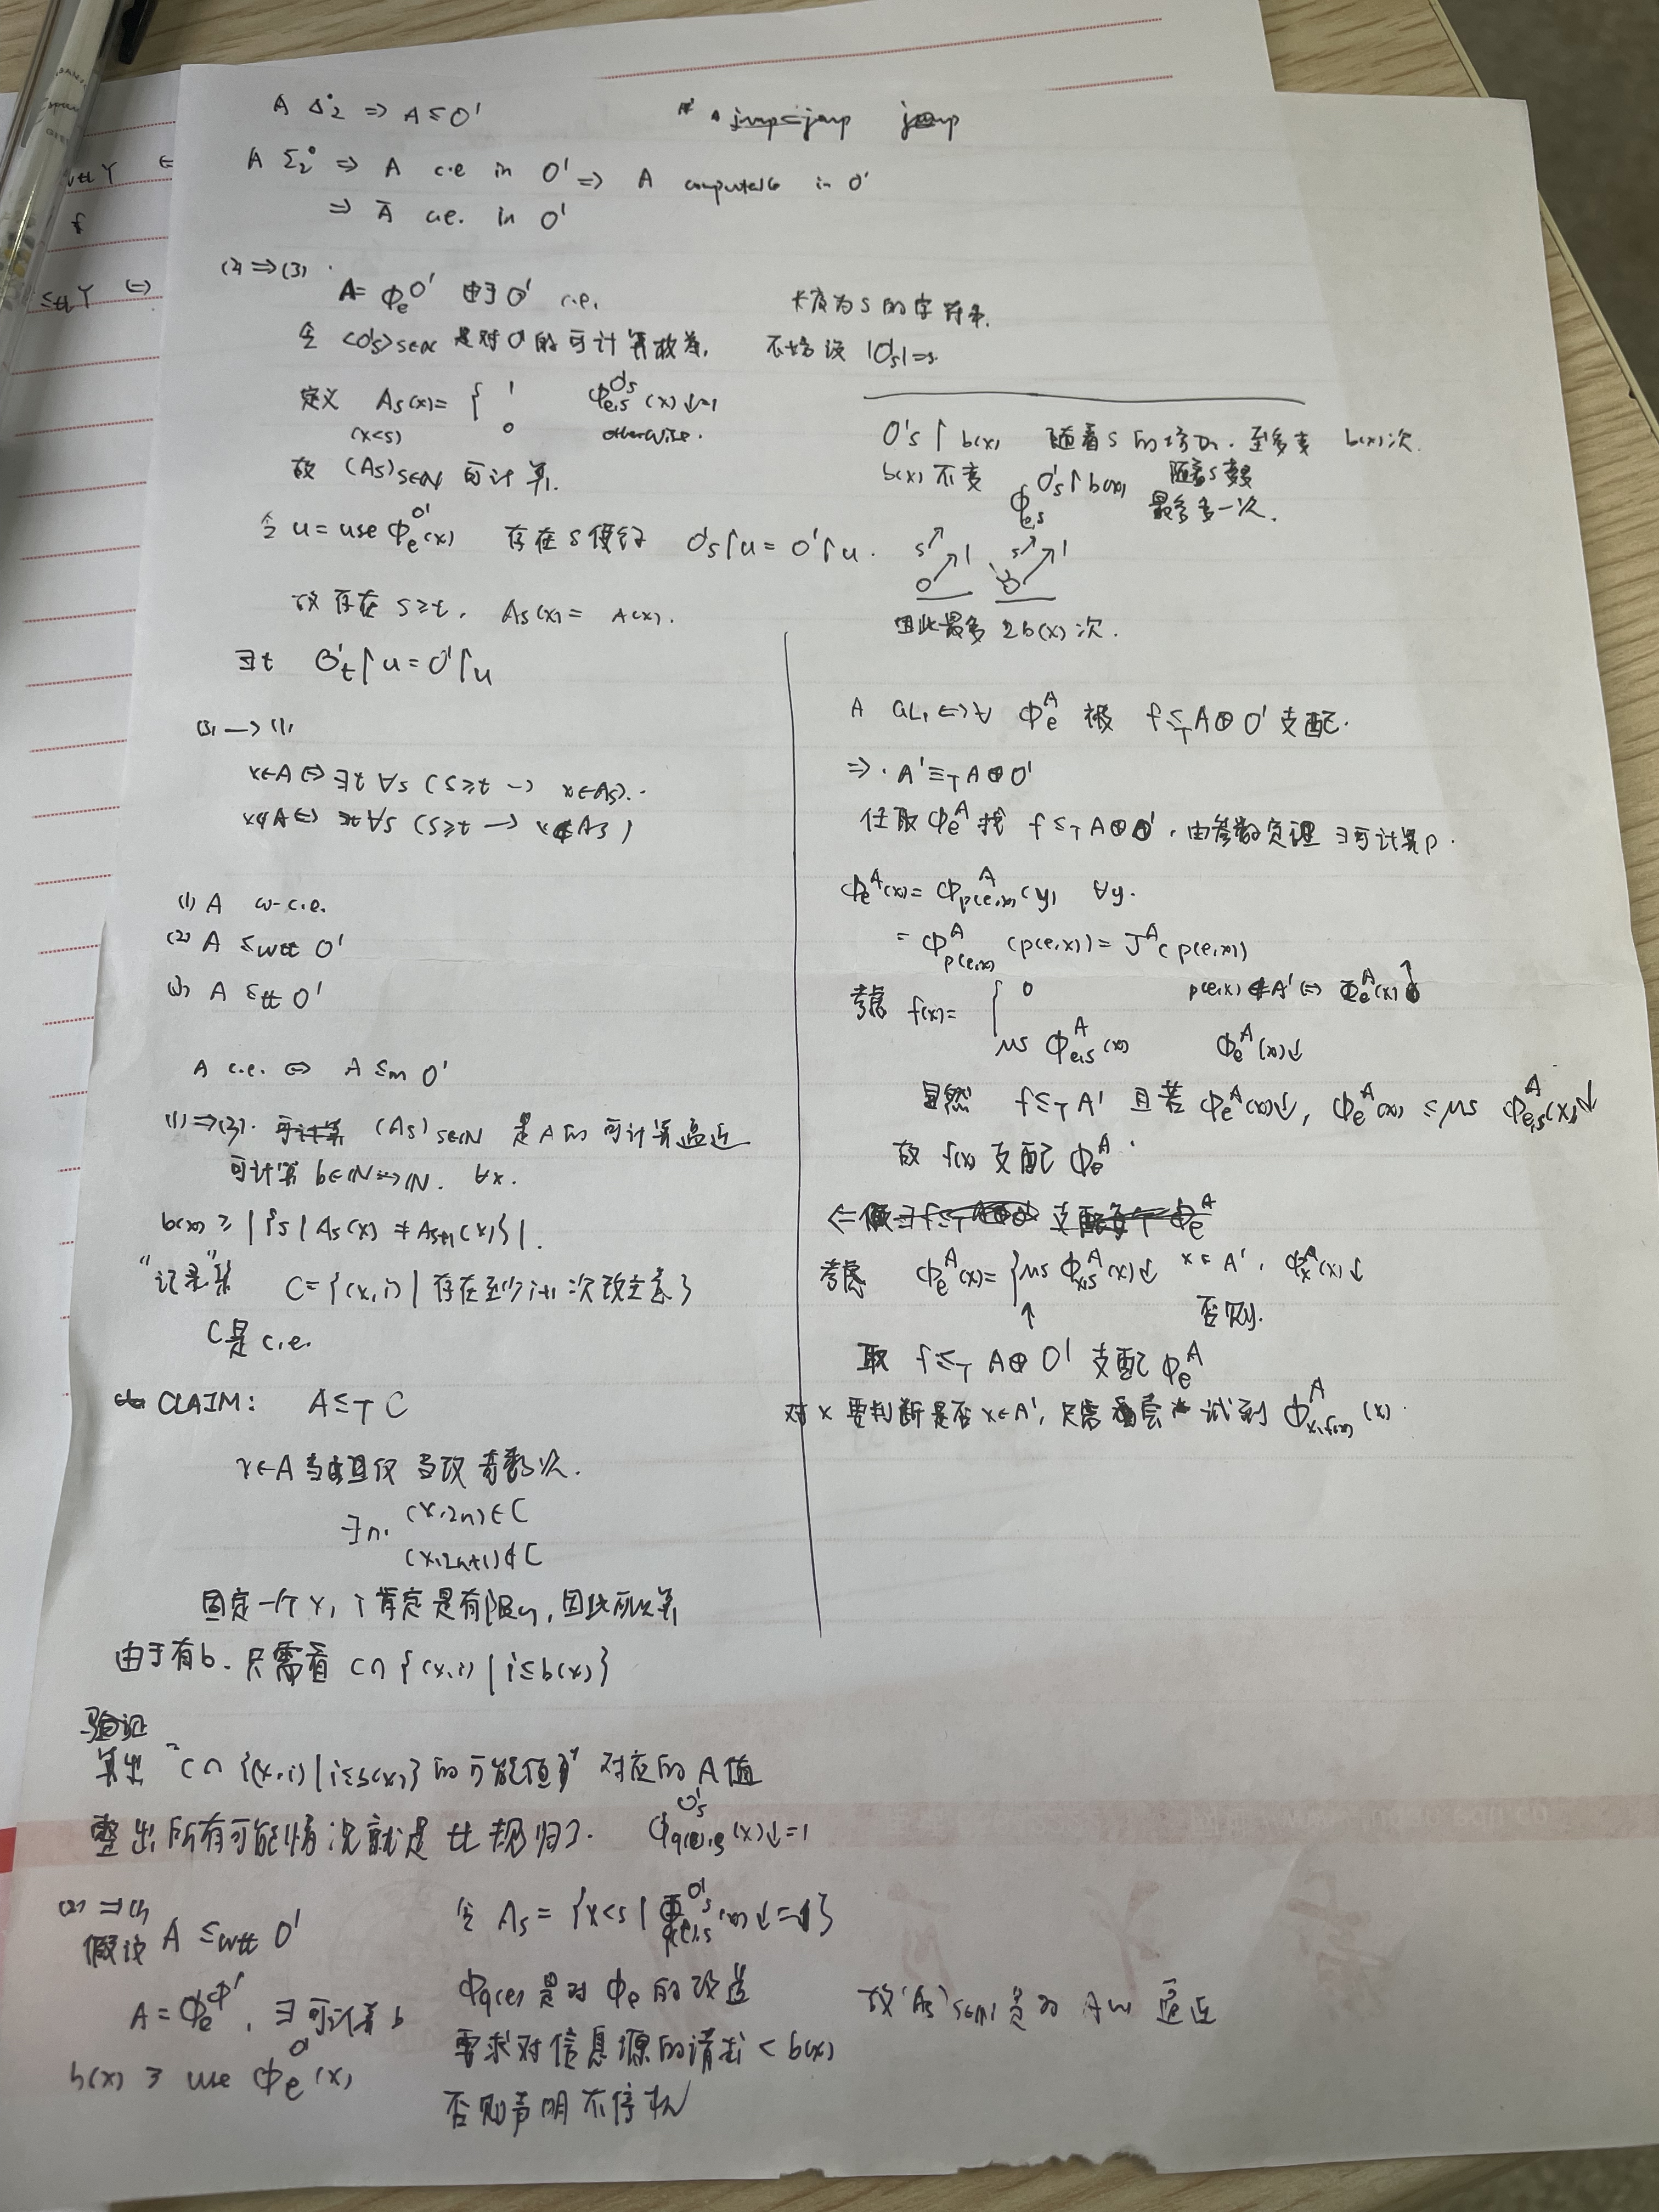
\includegraphics[width=.7\textwidth]{../images/Topology/1.png}
\end{center}

\begin{proof}
Let \(\calt\) denote the product topology on \(X\times Y\); let \(\calt'\) be the topology generated by \(\cals\).
Then \(\calt'\subset \calt\). On the other hand, every basis element \(U\times V\) for the topology \(\calt\) is a
finite intersection of elements of \(\cals\), since
\begin{equation*}
U\times V=\pi_1^{-1}\cap\pi_2^{-1}(V)
\end{equation*}
Hence \(U\times V\in\calt\)
\end{proof}


\subsection{The Subspace Topology}
\label{sec:org41d6913}
\begin{definition}[]
Let \(X\) be a topological space with topology \(\calt\). If \(Y\subseteq X\), then
\begin{equation*}
\calt_Y=\{Y\cap U\mid U\in\calt\}
\end{equation*}
is a topology on \(Y\), called the \textbf{subspace topology}. With this topology, \(Y\) is called a
\textbf{subspace} of \(X\)
\end{definition}

\begin{lemma}[]
if \(\calb\) is a basis for the topology of \(X\) then the collection
\begin{equation*}
\calb_Y=\{B\cap Y\mid B\in\calb\}
\end{equation*}
is a basis for the subspace topology on \(Y\)
\end{lemma}

\begin{proof}
Given \(U\) open in \(X\) and given \(y\in U\cap Y\), we can choose an element \(B\) of \(\calb\) s.t
. \(y\in B\subset U\). Then \(y\in B\cap Y\subset U\cap Y\). It follows from Lemma \ref{lemma13.2} that \(\calb_Y\) is a
basis for the subspace topology on \(Y\)
\end{proof}

\begin{lemma}[]
Let \(Y\) be a subspace of \(X\). If \(U\) is open in \(Y\) and \(Y\) is open in \(X\),
then \(U\) is open in \(X\)
\end{lemma}

\begin{theorem}[]
if \(A\) is a subspace of \(X\) and \(B\) is a subspace of \(Y\), then the product topology
on \(A\times B\) is the same as the topology \(A\times B\) inherits as a subspace of \(X\times Y\)
\end{theorem}

\begin{proof}
The set \(U\times V\) is the general basis element for \(X\times Y\), where \(U,V\) are open in \(X,Y\)
respectively.  Therefore \((U\times V)\cap(A\times B)\) is the general basis element for the subspace
topology on \(A\times B\). Now
 \begin{equation*}
(U\times V)\cap(A\times B)=(U\cap A)\times (V\cap B)
 \end{equation*}
\end{proof}

Now let \(X\) be an ordered set in the order topology, and let \(Y\) be a subset of \(X\). The
order relation on \(X\), when restricted to \(Y\), makes \(Y\) into an ordered set. However the
resulting order topology on Y need not be the same as the topology that Y inherits as a subspace
of X

\begin{examplle}[]
Consider the subset \(Y=[0,1]\) of the real line \(\R\) in the \emph{subspace} topology. Given \((a,b)\)
\begin{equation*}
(a,b)\cap Y=
\begin{cases}
&(a,b)\\
&[0,b)\\
&(a,1]\\
&Y\text{ or }\emptyset
\end{cases}
\end{equation*}
Sets of the second and third types are not open in the larger space \(\R\)

Note that these sets form a basis for the \emph{order}  topology on \(Y\). Thus we see that in the case
of the set \(Y=[0,1]\) its subspace topology and its order topology are the same
\end{examplle}

Given an ordered set \(X\), a subset \(Y\) of \(X\) is \textbf{convex} in \(X\) if for each pair of
points \(a<b\) of \(Y\), the entire interval \((a,b)\) of points of \(X\) lies in \(Y\). Note
that intervals and rays in \(X\) are convex in \(X\)

\begin{theorem}[]
Let \(X\) be an ordered set in the order topology; let \(Y\) be a subset of \(X\) that is convex
in \(X\). Then the order topology on \(Y\) is the same as the topology \(Y\) inherits as a
subspace of \(X\)
\end{theorem}

\begin{proof}
Consider the ray \((a,+\infty)\) in \(X\). If \(a\in Y\) then
\begin{equation*}
(a,+\infty)\cap Y=\{x\mid x\in Y\text{ and }x>a\}
\end{equation*}
this is an open ray of the ordered set \(Y\). If \(a\not\in Y\), then \(a\) is either a lower bound
on \(Y\) or an upper bound on \(Y\), since \(Y\) is convex. In the former case, \((a,+\infty)\cap Y=Y\);
in the latter case, it is empty

Similarly, \((-\infty,a)\cap Y\) is either an open ray of \(Y\), or \(Y\) itself, or empty. Since the
sets \((a,+\infty)\cap Y\) and \((-\infty,a)\cap Y\) form a subbasis for the subspace topology on \(Y\), and
since each is open in the order topology,and since each is open in the order topology,
the order topology contains the subspace topology

To prove the reverse, note that any open ray of \(Y\) equals the intersection of an open ray
of \(X\) with \(Y\), so it is open in the subspace topology on \(Y\). Since the open rays
of \(Y\) are a subbasis for the order topology, this topology is contained in the subspace topology
\end{proof}

\begin{exercise}
\label{15.1}
Show that if \(Y\) is a subspace of \(X\) and \(A\) is a subset of \(Y\), then the topology \(A\)
inherits as a subspace of \(Y\) is the same as the topology it inherits as a subspace of \(X\)
\end{exercise}

\begin{proof}
For every open set \(U\) of topology of \(X\), \(A\cap(Y\cap U)=A\cap U\).
\end{proof}

\begin{exercise}
\label{ex15.7}
Let \(X\) be an ordered set. If \(Y\) is a proper subset of \(X\) that is convex in \(X\), does
it follow that \(Y\) is an interval or a ray in \(X\)
\end{exercise}

\begin{proof}
Consider \((-\sqrt{2},\sqrt{2})\cap\Q\) which is convex in \(\Q\) but not an interval or a ray
\end{proof}


\subsection{Closed Sets and Limit Points}
\label{sec:orgc43c492}
A subset \(A\) of a topological space \(X\) is said to be \textbf{closed} if the set \(X-A\) is open

\begin{theorem}[]
Let \(X\) be a topological space. Then the following conditions hold:
\begin{enumerate}
\item \(\emptyset\) and \(X\) are closed
\item Arbitrary intersection of closed sets are closed
\item Finite unions of closed sets are closed
\end{enumerate}
\end{theorem}

\begin{theorem}[]
\label{thm17.2}
let \(Y\) be a subspace of \(X\). Then a set \(A\) is closed in \(Y\) iff it equals the
intersection of a closed set of \(X\) with \(Y\)
\end{theorem}

\begin{proof}
Assume that \(A=C\cap Y\), where \(C\) is closed in \(X\). Then \(X-C\) is open in \(X\), so
that \((X-C)\cap Y\) is open in \(Y\). But \((X-C)\cap Y=Y-A\). Hence \(Y-A\) is open  in \(Y\)

Assume that \(A\) is closed in \(Y\). Then \(Y-A=U\cap Y\) for some open set \(U\) in \(X\) and \(A=Y\cap(X-U)\)
\end{proof}

\begin{theorem}[]
Let \(Y\) be a subspace of \(X\). If \(A\) is closed in \(Y\) and \(Y\) is closed in \(X\),
then \(A\) is closed in \(X\)
\end{theorem}

Given a subset \(A\) of a topological space \(X\), the \textbf{interior} of \(A\) is defined as the union
of all open sets contained in \(A\), and the \textbf{closure} of \(A\) is defined as the intersection of
all closed sets containing \(A\) (\(\barA\))

\begin{theorem}[]
Let \(Y\) be a subspace of \(X\); let \(A\) be a subset of \(Y\); let \(\barA\) denote the
closure of \(A\) in \(X\). Then the closure of \(A\) in \(Y\) equals \(\barA\cap Y\)
\end{theorem}

\begin{proof}
Let \(B\) denote the closure of \(A\) in \(Y\). The set \(\barA\) is closed in \(X\),
so \(\barA\cap Y\) is closed in \(Y\) by Theorem \ref{thm17.2}. We have \(B\subset(\barA\cap Y)\)

On the other hand, \(B=C\cap Y\) for some \(C\) closed in \(X\). Then \(C\) is a closed set of \(X\)
containing \(A\).
\end{proof}

A set \(A\) \textbf{intersects} a set \(B\) if the intersection \(A\cap B\) is not empty

\begin{theorem}[]
\label{thm17.5}
Let \(A\) be a subset of the topological space \(X\)
\begin{enumerate}
\item \(x\in\barA\) iff every open set \(U\) containing \(x\) intersects \(A\)
\item Suppose the topology of \(X\) is given by a basis, then \(x\in\barA\) iff every basis
element \(b\) containing \(x\) intersects \(A\)
\end{enumerate}
\end{theorem}

\begin{proof}
\begin{enumerate}
\item We consider

\(x\not\in\barA\) iff there exists an open set \(U\) containing \(x\) that does not
intersects \(A\)

If \(x\not\in\barA\), the set \(U=X-\barA\) is an open set containing \(x\) that does not
intersects \(A\), as desired. Conversely, if there exsits an open set \(U\) containing \(x\)
which does not intersects \(A\), then \(X-U\) is a closed set containing \(A\).
Hence \(\barA\subseteq X-U\) and therefore \(x\not\in\barA\)
\end{enumerate}
\end{proof}

\(U\) is an open set containing \(x\) equals \(U\) is a \textbf{neighborhood} of \(x\)

\begin{examplle}[]
Let \(X\) be the real line \(\R\). If \(A=(0,1]\) then \(\barA=[0,1]\) for every neighborhood
of \(0\) intersects \(A\), while every point outside \([0,1]\) has a neighborhood disjoint
from \(A\).

If \(B=\{1/n\mid n\in\Z_+\}\) then \(\barB=\{0\}\cup B\). If \(C=\{0\}\cup(1,2)\) then \(\barC=\{0\}\cup[1,2]\). Also \(\bar{\Q}=\R\).
\end{examplle}

If \(A\)is a subset of the topological space \(X\) and if \(x\) is a point of \(X\), we say
that \(x\) is a \textbf{limit point} of \(A\) if every neighborhood of \(x\) intersects \(A\) in some
point \emph{other than \(x\) itself}. Said differently, \(x\) is a limit point of \(A\) if it belongs to
the closure of \(A-\{x\}\)

\begin{theorem}[]
Let \(A\) be a subset of the topological space \(X\); let \(A'\) be the set of all limit points
of \(A\). Then
\begin{equation*}
\barA=A\cup A'
\end{equation*}
\end{theorem}

\begin{proof}
By Theorem \ref{thm17.5} \(A'\subset\barA\).

Suppose \(x\in\barA-A\). Then \(x\in A'\)
\end{proof}

\begin{corollary}[]
A subset of a topological space is closed iff it contains all its limit points
\end{corollary}

\begin{proof}
\(A\) is closed iff \(\barA=A\)
\end{proof}

In the spaces \(\R\) and \(\R^2\) each one-point set \(\{x_0\}\) is closed since every point different
from \(x_0\) has a neighborhood not intersecting \(\{x_0\}\), so that \(\{x_0\}\) is its own
closure. But this fact is not true for arbitrary topological spaces. Consider the topology on the
three-point set \(\{a,b,c\}\) indicated in Figure \ref{fig:17.3}. The one-point set \(\{b\}\) is not
closed, for its complement is not open

\begin{figure}[htbp]
\centering
\includegraphics[width=.3\textwidth]{../images/Topology/2.png}
\caption{\label{fig:17.3}we}
\end{figure}

\index{converge}
In an arbitrary topological space, one says that a sequence \(x_1,x_2,\dots\) of points of the
space \(X\) \textbf{converges} to the point \(x\) of \(X\) provided that, corresponding to each
neighborhood \(U\) of \(x\) there is a positive integer \(N\) s.t. \(x_n\in U\) for all \(n\ge N\).
In \(\R\) and \(\R^2\) a sequence cannot converge to more than one point, but in an arbitrary space,
it can. In Figure \ref{fig:17.3} the sequence defined by setting \(x_n=b\) converges not only to
the point \(b\) but also to the point \(a\) and \(c\).

\begin{definition}[]
A topological space \(X\) is called a \textbf{Hausdorff space} if for each pair \(x_1,x_2\) of disjoint
points of \(X\), there exist neighborhoods \(U_1\) and \(U_2\) of \(x_1\) and \(x_2\) respectively,
that are disjoint
\end{definition}

\begin{theorem}[]
Every fintie point set in a Hausdorff space \(X\) is closed.
\end{theorem}

\begin{proof}
It suffices to show that every one-point set \(\{x_0\}\) is closed.
\end{proof}

The condition that finite point sets be closed is in fact weaker than the Hausdorff condition.
For example, the real line \(\R\) in the finite complement topology is not a Hausdorff space, but
it is a space in which finite point sets are closed. The condition that finite point sets be
closed is called the \textbf{\(T_1\) axiom}

\begin{theorem}[]
Let \(X\) be a space satisfying the \(T_1\) axiom; let \(A\) be a subset of \(X\). Then the
point \(x\) is a limit point of \(A\) iff every neighborhood of \(x\) contains infinitely many points
\end{theorem}

\begin{proof}
If \(x\) is a limit point of \(A\) and suppose some neighborhood \(U\) of \(x\) intersects \(A\)
in only finitely many points. Then \(U\) also intersects \(A-\{x\}\) in finitely many points;
let \(\{x_1,\dots,x_m\}\) be the points of \(U\cap(A-\{x\})\). The set \(X-\{x_1,\dots,x_m\}\) is an open set
of \(X\), then
\begin{equation*}
U\cap(X-\{x_1,\dots,x_m\})
\end{equation*}
is a neighborhood of \(x\) that intersects the set \(A-\{x\}\)
\end{proof}

\begin{theorem}[]
If \(X\) is the Hausdorff space, then a sequence of points of \(X\) converges to at most one
point of \(X\)
\end{theorem}

\begin{proof}
Suppose that \(x_n\) is a sequence of points of \(X\) that converges to \(x\). If \(y\neq x\)
let \(U\) and \(V\) be disjoint neighborhoods of \(x\) and \(y\) respectively. Since \(U\)
contains \(x_n\) for all but finitely many values of \(n\), the set \(V\) cannot.
Therefore \(x_n\) cannot converge to \(y\).
\end{proof}

If the sequence \(x_n\) of points of the Hausdorff space \(X\) converges to the point \(x\)
of \(X\), we often write \(x_n\to x\) and we say that \(x\) is the \textbf{limit} of the sequence \(x_n\)

\begin{theorem}[]
Every simply ordered set is a Hausdorff space in the order topology. The product of two Hausdorff
spaces is a Hausdorff space. A subspace of a Hausdorff space is a Hausdorff space.
\end{theorem}

\begin{exercise}
\label{ex17.5}
Let \(X\) be an ordered set in the order topology. Show that \(\ove{(a,b)}\subset[a,b]\). Under what
conditions does equality hold
\end{exercise}

\begin{proof}
It equals the closure iff both endpoints are limit points of the interval, i.e. if \((a,b)\) is not
empty and for every \(x\in(a,b)\) there are \(s,t\in(a,b)\) such that \(a<s<x<t<b\) . This is equivalent to the
requirement that \(a\) has no immediate successor, and \(b\) has no immediate predecessor. Otherwise, if
\(a\) has an immediate successor \(c\) then \((−∞,c)\) is an open set containing \(a\) that does not intersect
\((a,b)\) , and, similarly, if \(b\) has an immediate predecessor \(c\) then \((c,+∞)\) is an open set containing
\(b\) that does not intersect \((a,b)\) .
\end{proof}

\begin{exercise}
\label{ex17.6}
Let \(A\),\(B\) and \(A_\alpha\) denote subsets of a space \(X\). Prove the following
\begin{enumerate}
\item If \(A\subset B\) then \(\barA\subset\barB\)
\item \(\ove{A\cup B}=\barA\cup\barB\)
\item \(\ove{\bigcup A_\alpha}\supset\bigcup\barA_\alpha\); give an example where equality fails
\end{enumerate}
\end{exercise}

\begin{proof}
\begin{enumerate}
\setcounter{enumi}{1}
\item Suppose \(x\not\in\barA\cup\barB\). By Theorem \ref{thm17.5} there is a neiborhoods \(U_A,U_B\)
of \(x\) s.t. \(U_A\cap A=U_B\cap B=\emptyset\).  Let \(U=U_A\cap U_B\). Then \(U\cap(A\cup B)=\emptyset\).
\item Consider \(A_n=(1/n,2]\) for \(n\in\Z_+\)
\end{enumerate}
\end{proof}

\begin{exercise}
\label{ex17.8}
Let \(A\),\(B\) and \(A_\alpha\) denote subsets of a space \(X\). Determine whether the following
equations hold
\begin{enumerate}
\item \(\ove{A\cap B}=\barA\cap\barB\)
\item \(\ove{\bigcap A_\alpha}=\bigcap\barA_\alpha\)
\item \(\ove{A-B}=\barA-\barB\)
\end{enumerate}
\end{exercise}

\begin{proof}
\begin{enumerate}
\item Consider \(A=(1,2)\) and \(B=(0,1)\) in \(\R\). We only have \(\ove{A\cap B}\subset\barA\cap\barB\)
\setcounter{enumi}{2}
\item \(\ove{A-B}\supset\barA-\barB\). \(A=(0,2),B=(0,1)\)
\end{enumerate}
\end{proof}

\begin{exercise}
\label{ex17.13}
\(X\) is Hausdorff iff the \textbf{diagonal} \(\Delta=\{x\times x\mid x\in X\}\) is closed in \(X\times X\).
\end{exercise}

\begin{proof}
\(\Delta\) is closed in \(X\times X\) iff for \(x\neq y\) there is a basis \(x\times y\in U\times V\subset X\times X\)
where  \(U\) and \(V\) are neighborhoods of \(x\) and \(y\) respectively s.t. no
points \((z,z)\in U\times V\)
iff any pair of of different points having disjoint neighborhoods
\end{proof}

\subsection{Continuous Functions}
\label{sec:org921dfb3}
Let \(X\) and \(Y\) be topological spaces. A function \(f:X\to Y\) is said to be \textbf{continuous} if for
each open subset \(V\) of \(Y\) the set \(f^{-1}(V)\) is an open subset of \(X\).

Let's note that if the topology of the range space \(Y\) is given by a basis \(\calb\), then to prove
continuity of \(f\) it suffices to show that the inverse image of every \emph{basis element} is oepn.

If the topology on \(Y\) is given by a subbasis \(\cals\), to prove continuity of \(f\) it will even
suffice to show that the inverse of each \emph{subbasis} element is open.

\begin{examplle}[]
Let's consider a function
\begin{equation*}
f:\R\to\R
\end{equation*}

Now we prove that our definition implies the \(\epsilon\)-\(\delta\) definition

Given \(x_0\in\R\)  and given \(\epsilon>0\) the interval \(V=(f(x_0)-\epsilon,f(x_0)+\epsilon)\) is an open set of the
range space \(\R\). Therefore, \(f^{-1}(V)\) is an open set in the domain space \(\R\).
Because \(x_0\in f^{-1}(V)\), it contains some basis element \((a,b)\) about \(x_0\). We choose
\(\delta\) to be the smaller of the two numbers \(x_0-a\) and \(b-x_0\). Then if \(\abs{x-x_0}<\delta\), the
point \(x\) must be in \((a,b)\), so that \(f(x)\in V\) and \(\abs{f(x)-f(x_0)}<\epsilon\) as desired
\end{examplle}

\begin{examplle}[]
Let \(\R\) denote the set of real numbers in its usual topology. Let
\begin{equation*}
f:\R\to\R_l
\end{equation*}
by the identity function \(f(x)=x\). Then \(f\) is not a continuous function. However
\begin{equation*}
g:\R_l\to\R
\end{equation*}
is continuous
\end{examplle}

\begin{theorem}[]
Let \(X\) and \(Y\) be topological spaces: let \(f:X\to Y\). TFAE
\begin{enumerate}
\item \(f\) is continuous
\item for every \(A\subseteq X\), \(f(\barA)\subset\ove{f(A)}\)
\item for every closed set \(B\) of \(Y\), the set \(f^{-1}(B)\) is closed in \(X\)
\item for each \(x\in X\) and each neiborhood \(V\) of \(f(x)\), there is a neighborhood \(U\)
of \(x\) s.t. \(f(U)\subset V\)
\end{enumerate}


If the condition 4 holds for the point \(x\) of \(X\), we say that \(f\) is \textbf{continuous at the
point \(x\)}
\end{theorem}

\begin{proof}
\(1\to 2\). Assume \(f\) is continuous. Let \(A\subseteq X\) and \(x\in\barA\). Let \(V\) be a neighborhood
of \(f(x)\). Then \(f^{-1}(V)\) is an open set of \(X\) containing \(x\);  it must
intersect \(A\) in some point \(y\). Then \(V\) intersects \(f(A)\) in the point \(f(y)\), so
that \(f(x)\in\ove{f(A)}\)

\(2\to 3\). Let \(B\) be closed in \(Y\) and let \(A=f^{-1}(B)\). We show that \(\barA=A\). We have
\(f(A)=f(f^{-1}(B))\subset B\). Therefore if \(x\in\barA\)
\begin{equation*}
f(x)\in f(\barA)\subset\ove{f(A)}\subset\barB=B
\end{equation*}
so that \(x\inf^{-1}(B)=A\)

\(3\to 1\). easy

\(1\to 4\). easy

\(4\to 1\). not hard \emoji{😊}
\end{proof}

let \(X\) and \(Y\) be topological spaces; let \(f:X\to Y\) be a bijection. If both the
function \(f\) and the inverse function
\begin{equation*}
f^{-1}:Y\to X
\end{equation*}
are continuous, then \(f\) is called a \textbf{homeomorphism}

Suppose that \(f:X\to Y\) is an injective continuous map, where \(X\) and \(Y\) are topological
spaces. Let \(Z\) be the image set \(f(X)\), considered as a subspace of \(Y\); then the
function \(f':X\to Z\) obtained by restricting the range of \(f\)  is bijectiive. If \(f'\) happens
to be a homeomorphism of \(X\) with \(Z\), we say that the map \(f:X\to Y\) is a
\textbf{topological embedding} or simpy an \textbf{embedding} of \(X\) in \(Y\)

\begin{examplle}[]
A bijectiive function \(f:X\to Y\) can be continuous without being a homeomorphism. One such
function is the identity map \(g:\R_l\to\R\)。 Another is the following:

Let \(S^1\) denote the \textbf{unit circle},
\begin{equation*}
S^1=\{x\times y\mid x^2+y^2=1\}
\end{equation*}
considered as a subspace of the plane \(\R^2\) and let
\begin{equation*}
f:[0,1)\to S^1
\end{equation*}
be the map defined by \(f(t)=(\cos 2\pi t,\sin2\pi t)\). \(f\) is continuous but not \(f^{-1}\). The
image under \(f\) of the open set \(U=[0,\frac{1}{4})\) of the domain is not open in \(S^1\), for
the point \(p=f(0)\) lies in no open set \(V\) of \(\R^2\) s.t. \(V\cap S^1\subset f(U)\)

\begin{figure}[htbp]
\centering
\includegraphics[width=.7\textwidth]{../images/Topology/3.png}
\label{}
\end{figure}
\end{examplle}


\begin{theorem}[Rules for constructing continuous functions]
Let \(X,Y\) and \(Z\) be topological spaces
\begin{enumerate}
\item (Constant function) if \(f:X\to Y\) maps all of \(X\) into the single point \(y_0\) of \(Y\),
then \(f\) is continuous
\item (Inclusion) If \(A\) is a subspace of \(X\), the inclusion function \(j:A\to X\) is continuous
\item (Composites) If \(f:X\to Y\) and \(g:Y\to Z\) are continuous, then the map \(g\circ f:X\to Z\) is continuous
\item (Restricting the domain) if \(f:X\to Y\) is continuous, and if \(A\) is a subspace of \(X\),
then the restricted function \(f|A:A\to Y\) is continuous
\item (Restricting or expanding the range) Let \(f:X\to Y\) be continuous. If \(Z\) is a subspace
of \(Y\) containing the image set \(f(X)\), then the function \(g:X\to Z\) obtained by
restricting the range of \(f\) is continuous. If \(Z\) is a space having \(Y\) as a subspace,
then the function \(h:X\to Z\) obtained by expanding the range of \(f\) is continuous
\item (Local formulation of continuity) The map \(f:X\to Y\) is continuous if \(X\) can be written as
the union of open sets \(U_\alpha\) s.t. \(f|U_\alpha\) is continuous for each \(\alpha\)
\end{enumerate}
\end{theorem}

\begin{proof}
\begin{enumerate}
\item Let \(V\) be open in \(Y\), then \(f^{-1}(V)\) equals \(\emptyset\) or \(X\)
\end{enumerate}
\end{proof}

\begin{theorem}[The pasting lemma]
Let \(X=A\cup B\), where \(A\) and \(B\) are closed in \(X\). Let \(f:A\to Y\) and \(g:B\to Y\) be
continuous. If \(f(x)=g(x)\) for every \(A\cap B\) then \(f\) and \(g\) combine to give a continuous
function \(h:X\to Y\), defined by setting \(h(x)=f(x)\) if \(x\in A\) and \(h(x)=g(x)\) if \(x\in B\)
\end{theorem}

The open set case of the pasting lemma is just the local formulation of continuity

\begin{theorem}[Maps into products]
Let \(f:A\to X\times Y\) be given by the equation
\begin{equation*}
f(a)=(f_1(a),f_2(a))
\end{equation*}
Then \(f\) is continuous iff the functions
\begin{equation*}
f_1:A\to X \quad\text{ and }\quad f_2:A\to Y
\end{equation*}
are continuous

The maps \(f_1\) and \(f_2\) are called the \textbf{coordinate functions}
\end{theorem}

\begin{proof}
First note that \(\pi_1,\pi_2\) are continuous. For \(\pi_1^{-1}(U)=U\times Y\) and \(\pi_2^{-1}(V)=X\times V\) and
these sets are open if \(U\) and \(V\) are open. Note that for each \(a\in A\)
\begin{equation*}
f_1(a)=\pi_1(f(a))\quad\text{ and }\quad f_2(a)=\pi_2(f(a))
\end{equation*}
If \(f\) is continuous, then \(f_1,f_2\) are continuous

Conversely, we show that for each basis element \(U\times V\) for the topology \(X\times Y\) its inverse
image \(f^{-1}(U\times V)\) is open. \(a\in f^{-1}(U\times V)\) iff \(f(a)\in(U\times V)\) iff \(f_1(a)\in U\)
and \(f_2(a)\in V\). Therefore
\begin{equation*}
f^{-1}(U\times V)=f_1^{-1}(U)\times f_2^{-1}(V)
\end{equation*}
\end{proof}

\begin{exercise}
\label{ex18.11}
Let \(F:X\times Y\to Z\). We say that \(F\) is \textbf{continuous in each variable separately} if for
each \(y_0\) in \(Y\), the map \(h:X\to Z\) defined by \(h(x)=F(x\times y_0)\) is continuous, and for
each \(x_0\) in \(X\), the map \(k:Y\to Z\) defined by \(k(y)=F(x_0\times y)\) is continuous. Show that
if \(F\) is continuous, then \(F\) is continuous in each variable separately.
\end{exercise}

\begin{exercise}
\label{ex18.12}
Let \(F:\R\times \R\to\R\) be defined by the equation
\begin{equation*}
F(x\times y)=
\begin{cases}
xy/(x^2+y^2)&\text{if }x\times y\neq 0\times 0\\
0
\end{cases}
\end{equation*}
\begin{enumerate}
\item Show that \(F\) is continuous in each variable separately
\item Compute the function \(g:\R\to\R\) defined by \(g(x)=F(x\times x)\)
\item Show that \(F\) is not continuous
\end{enumerate}
\end{exercise}

\subsection{The Product Topology}
\label{sec:org7d4323e}

\begin{definition}[]
Let \(J\) be an index set. Given a set \(X\), we define \textbf{\(J\)-tuple} of elements of \(X\) to be a
function \(\bx:J\to X\). If \(\alpha\) is an element of \(j\), we often denote the value of \(\bx\) at \(\alpha\)
by \(x_\alpha\); we call it the \(\alpha\)th \textbf{coordinate} of \(\bx\). And we often denote the function \(\bx\)
itself by the symbol
\begin{equation*}
(x_\alpha)_{\alpha\in J}
\end{equation*}
We denote the set of all \(J\)-tuples of elements of \(X\) by \(X^J\)
\end{definition}

\begin{definition}[]
Let \(\{A_\alpha\}_{\alpha\in J}\) be an indexed family of sets; let \(X=\bigcup_{\alpha\in J}A_\alpha\). The \textbf{cartesian product}
of this indexed family, denoted by
\begin{equation*}
\prod_{\alpha\in J}A_\alpha
\end{equation*}
is defined to be the set of all \(J\)-tuples \((x_\alpha)_{\alpha\in J}\) of elements of \(X\)
s.t. \(x_\alpha\in A_\alpha\)  for each \(\alpha\in J\). That is, it is the set of all functions
\begin{equation*}
\bx:J\to\bigcup_{\alpha\in J}A_\alpha
\end{equation*}
s.t. \(\bx(\alpha)\in A_\alpha\) for each \(\alpha\in J\)
\end{definition}

\begin{definition}[]
Let \(\{X_\alpha\}_{\alpha\in J}\) be an indexed family of topological spaces. Let us take as a basis for a
topology on the product space
\begin{equation*}
\prod_{\alpha\in J}X_\alpha
\end{equation*}
the collection of all sets of the form
\begin{equation*}
\prod_{\alpha\in J}U_\alpha
\end{equation*}
where \(U_\alpha\) is open in \(X_\alpha\), for each \(\alpha\in J\). The topology generated by this basis is
called the \textbf{box topology}
\end{definition}

Now we generalize the subbasis formulation of the definition. Let
\begin{equation*}
\pi_\beta:\prod_{\alpha\in J}X_\alpha\to X_\beta
\end{equation*}
be the function assigning to each element of the product space its \(\beta\)th coordinate
\begin{equation*}
\pi_\beta((x_\alpha)_{\alpha\in J})=x_\beta
\end{equation*}
it is called the \textbf{projection mapping} associated with the index \(\beta\)

\begin{definition}[]
Let \(\cals_\beta\) denote the collection
\begin{equation*}
\cals_\beta=\{\pi_\beta^{-1}(U_\beta)\mid U_\beta\text{ open in }X_\beta\}
\end{equation*}
and let \(\cals\) denote the union of these collections
\begin{equation*}
\cals=\bigcup_{\beta\in J}\cals_\beta
\end{equation*}
The topology generated by the subbasis \(\cals\)  is called the \textbf{product topology}. In this
topology \(\prod_{\alpha\in J}X_\alpha\) is called a \textbf{product space}
\end{definition}

To compare these topologies, we consider the basis \(\calb\) that \(\cals\) generates. The
collection \(\calb\) consists of all finite intersections of elements of \(\cals\). If we intersect
elements belonging to the same one of the sets \(\cals_\beta\) we do not get anything new, because
\begin{equation*}
\pi_\beta^{-1}(U_\beta)\cap\pi_\beta^{-1}(V_\beta)=\pi_\beta^{-1}(U_\beta\cap V_\beta)
\end{equation*}
We get something new only when we intersect elements from different sets \(\cals_\beta\). Thus the typical
element of the basis \(\calb\) can be described as follows: let \(\beta_1,\dots,\beta_n\) be a finite set of
distinct indices from the index set \(J\), and let \(U_{\beta_i}\) be an open set in \(X_{\beta_i}\)
for \(i=1,\dots,n\). Then
\begin{equation*}
B=\pi_{\beta_1}^{-1}(U_{\beta_1})\cap\dots\cap\pi_{\beta_n}^{-1}(U_{\beta_n})
\end{equation*}
is the typical element of \(\calb\)

Now a point \(\bx=(x_\alpha)\) is in \(B\) iff its \(\beta_1\)th coordinate is in \(U_{\beta_1}\),  its \(\beta_2\)th
coordinate is in \(U_{\beta_2}\), and so on. As a result, we can write \(B\) as the product
\begin{equation*}
B=\prod_{\alpha\in J}U_\alpha
\end{equation*}
where \(U_\alpha\) denotes the entire space \(X_\alpha\) if \(\alpha\neq\beta_1,\dots,\beta_n\)

\begin{theorem}[Comparison of the box and product topologies]
The box topology on \(\prod X_\alpha\) has as basis all sets of the form \(\prod U_\alpha\), where \(U_\alpha\) is open
in \(X_\alpha\) for each \(\alpha\). The product topology on \(\prod X_\alpha\) has as basis all sets of the
form \(U_\alpha\), where \(U_\alpha\) is open in \(U_\alpha\) for  each \(\alpha\) and \(U_\alpha\) equals \(X_\alpha\) except
for finitely many values of \(\alpha\)
\end{theorem}

\begin{quoting}
Whenever we consider the product \(X_\alpha\), we shall assume it is given the product topology unless
we specifically state otherwise.
\end{quoting}

\begin{theorem}[]
\label{thm19.2}
Suppose the topology on each space \(X_\alpha\) is given by a basis \(\calb_\alpha\). The collection of all
sets of the form
\begin{equation*}
\prod_{\alpha\in J}B_\alpha
\end{equation*}
where \(B_\alpha\in \calb_\alpha\) for each \(\alpha\), will serve as a basis for the box topology on \(\prod_{\alpha\in J}X_\alpha\)

The collection of all sets of the same form, where \(B_\alpha\in\calb_\alpha\) for finitely many indices \(\alpha\)
and \(B_\alpha=X_\alpha\) for all the remaining indices, will serve as a basis for the product
topology \(\prod_{\alpha\in J}X_\alpha\)
\end{theorem}

\begin{theorem}[]
\label{thm19.3}
Let \(A_\alpha\) be a subspace of \(X_\alpha\) for each \(\alpha\in J\). Then \(\prod A_\alpha\) is a subspace of \(\prod X_\alpha\)
is both products are given the box topology or product topology
\end{theorem}

\begin{theorem}[]
\label{thm19.4}
If each space \(X_\alpha\) is a Hausdorff space, then \(\prod X_\alpha\) is a Hausdorff space in both the box
and product topologies
\end{theorem}

\begin{theorem}[]
\label{thm19.5}
Let \(\{X_\alpha\}\) be an indexed family of spaces; let \(A_\alpha\subseteq X_\alpha\)  for each \(\alpha\). If \(\prod X_\alpha\) is given
either the product or the box topology, then
\begin{equation*}
\prod \barA_\alpha=\ove{\prod A_\alpha}
\end{equation*}
\end{theorem}

\begin{proof}
Let \(\bx=(x_\alpha)\) be a point of \(\prod\barA_\alpha\); we show that \(\bx\in\ove{\prod A_\alpha}\). Let \(U=\prod U_\alpha\)  be a
basis element for either the box or product topology that contains \(\bx\). Since \(x_\alpha\in\barA_\alpha\),
we can choose a point \(y_\alpha\in U_\alpha\cap A_\alpha\). Then \(\by=(y_\alpha)\) belongs to both \(U\) and \(\prod A_\alpha\).
Since \(U\) is arbitrary, it follows that \(\bx\in\prod A_\alpha\)

Conversely, suppose \(\bx=(x_\alpha)\) lies in the closure of \(\prod A_\alpha\), in either topology. We show
that for any given index \(\beta\), we have \(x_\beta\in\barA_\beta\). Let \(V_\beta\) be an arbitrary open set of \(X_\beta\)
containing \(x_\beta\). Since \(\pi_\beta^{-1}(V_\beta)\) is open in \(\prod X_\alpha\) in either topology, it contains a
point \(\by=(y_\alpha)\) of \(\prod A_\alpha\). Then \(y_\beta\) belongs to \(V_\beta\cap A_\beta\). It follows that \(x_\beta\in\barA_\beta\)
\end{proof}

\begin{theorem}[]
\label{thm19.6}
Let \(f:A\to\prod_{\alpha\in J}X_\alpha\) be given by the equation
\begin{equation*}
f(a)=(f_\alpha(a))_{\alpha\in J}
\end{equation*}
where \(f_\alpha:A\to X_\alpha\) for each \(\alpha\). Let \(\prod X_\alpha\) have the product topology. Then the function \(f\)
is continuous iff each function \(f_\alpha\) is continuous
\end{theorem}

\begin{proof}
\(\Rightarrow\) composition of continuous functions is continuous

\(\Leftarrow\) Suppose that each coordinate function \(f_\alpha\) is continuous. To prove that \(f\) is
continuous, it suffices to prove that the inverse image under \(f\) of each subbasis element is
open in \(A\).  A typical subbasis element for the
product topology on \(\prod X_\alpha\) is a set of the form \(\pi_\beta^{-1}(U_\beta)\) where \(\beta\) is some index
and \(U_\beta\) is open in \(X_\beta\). now
\begin{equation*}
f^{-1}(\pi_\beta^{-1}(U_\beta))=f_\beta^{-1}(U_\beta)
\end{equation*}
because \(f_\beta=\pi_\beta\circ f\). Since \(f_\beta\) is continuous, this set is open in \(A\)
\end{proof}

\begin{examplle}[]
Consider \(\R^\omega\) and define \(f:\R\to\R^\omega\)
\begin{equation*}
f(t)=(t,t,\dots)
\end{equation*}
\(f\) is continuous if \(\R^\omega\) is given the box topology. Consider the basis element
\begin{equation*}
B=(-1,1)\times(-\frac{1}{2},\frac{1}{2})\times(-\frac{1}{3},\frac{1}{3})\times\dots
\end{equation*}
We assert that \(f^{-1}(B)\) is not open in \(\R\). \(f^{-1}(B)=\{0\}\)
\end{examplle}

\begin{exercise}
\label{ex19.6}
let \(\bx_1,\bx_2,\dots\) be a sequence of the points of the products space \(\prod X_\alpha\). Show that this
sequence converges to the point \(\bx\) iff the sequence \(\pi_\alpha(\bx_1),\pi_\alpha(\bx_2),\dots\) converges
to \(\pi_\alpha(\bx)\) for each \(\alpha\)
\end{exercise}

\begin{proof}
Given a neighborhood \(U=\prod U_\alpha\) of \(\bx\), for each \(\alpha\), we have \(N_\alpha\) s.t. \(\pi_\alpha(x_n)\in U_\alpha\) for
all \(n\ge N_\alpha\). If \(U_\alpha=X_\alpha\) we take \(N_\alpha=1\). Hence in product topology we have only finitely
many \(N_\alpha>1\) and we can take max. This fails in box topology as it might not have max
\end{proof}

\begin{exercise}
\label{ex19.7}
Let \(\R^\infty\) be the subset of \(\R^\omega\) consisting of all sequences that are ``eventually zero'', that
is, all sequences \((x_1,x_2,\dots)\) s.t. \(x_i\neq0\) for only finitely many values of \(i\). What is
the closure of \(\R^\infty\) in \(\R^\omega\) in the box and product topologies? justify your answer
\end{exercise}

\begin{proof}
\(\ove{\R^\infty}=\R^\omega\) for both

If \(\R^\infty\) is given the product topology, given a point \(\bx\in\R^\omega\) and a neighborhood \(U=\bigcup_i U_i\)
where \(U_i\) is a proper open subset of \(\R\) for finitely many \(i\in\omega\). Choose \(y_i\in U_i\)
and \(y_j=0\) if \(U_j=\R\). Then \(\by\in\R^\infty\cap U\). Hence \(x\in\ove{\R^\infty}\)
\end{proof}

\begin{exercise}
Given sequences \((a_1,a_2,\dots)\) and \((b_1,b_2,\dots)\) of real numbers with \(a_i>0\) for all \(i\),
define \(h:\R^\omega\to\R^\omega\) by the equation
\begin{equation*}
h((x_1,x_2,\dots))=(a_1x_1+b_1,a_2x_2+b_2,\dots)
\end{equation*}
Show that if \(\R^\omega\) is given the product topology, \(h\) is a homeomorphism of \(\R^\omega\) with
itself. What happens if \(\R^\omega\) is given the box topology
\end{exercise}

\begin{proof}
both box and product
\end{proof}


\subsection{The Metric Topology}
\label{sec:org3959bd9}
\begin{definition}[]
A \textbf{metric} on a set \(X\) is a function
\begin{equation*}
d:X\times X\to R
\end{equation*}
having the following properties
\begin{enumerate}
\item \(d(x,y)\ge0\) for all \(x,y\in X\); equality holds iff \(x=y\)
\item \(d(x,y)=d(y,x)\) for all \(x,y\in X\)
\item \(d(x,y)+d(y,z)\ge d(x,z)\) for all \(x,y,z\in X\)
\end{enumerate}
\end{definition}

Given a metric \(d\) on \(X\), the number \(d(x,y)\) is often called the \textbf{distance} between \(x\)
and \(y\) in the metric \(d\). Given \(\epsilon>0\) consider the set
\begin{equation*}
B_d(x,\epsilon)=\{y\mid d(x,y)<\epsilon\}
\end{equation*}
of all points \(y\) whose distance from \(x\) is less than \(\epsilon\). It is called the \textbf{\(\epsilon\)-ball
centered at \(x\)}

\begin{definition}[]
If \(d\) is a metric on the set \(X\), then the collection of all \(\epsilon\)-balls \(B_d(x,\epsilon)\)
for \(x\in X\) and \(\epsilon>0\) is a basis for a topology on \(X\), called the \textbf{metric topology} induced
by \(d\)
\end{definition}

Check the second condition.

If \(y\in B(x,\epsilon)\) then there is a basis element \(B(y,\delta)\) \emph{centered} at \(y\) that is contained
in \(B(x,\epsilon)\). Define \(\delta\) to be \(\epsilon-d(x,y)\). Then \(B(y,\delta)\subset B(x,\epsilon)\), for if \(z\in B(y,\delta)\)
then \(d(y,z)<\epsilon-d(x,y)\), from which we conclude that
\begin{equation*}
d(x,z)\le d(x,y)+d(y,z)<\epsilon
\end{equation*}

\begin{figure}[htbp]
\centering
\includegraphics[width=.4\textwidth]{../images/Topology/4.png}
\label{}
\end{figure}

Let \(B_1\) and \(B_2\) be two basis element and let \(y\in B_1\cap B_2\).We have just shown that we can
choose positive numbers \(\delta_1\) and \(\delta_2\) so that \(B(y,\delta_1)\subset B_1\) and \(B(y,\delta_2)\subset B_2\).
Let \(\delta=\min\{\delta_1,\delta_2\}\) we conclude \(B(y,\delta)\subset B_1\cap B_2\). Hence
\begin{quoting}
A set \(U\) is open in the metric topology induced by \(d\) iff for each \(y\in U\) there is
a \(\delta>0\) s.t. \(B_d(y,\delta)\subset U\)
\end{quoting}
\end{document}
